\documentclass{standalone}
\usepackage{tikz}
\usepackage{ctex,siunitx}
\setCJKmainfont{Noto Serif CJK SC}
\usepackage{tkz-euclide}
\usepackage{amsmath}
\usepackage{wasysym}
\usetikzlibrary{patterns, calc}
\usetikzlibrary {decorations.pathmorphing, decorations.pathreplacing, decorations.shapes,}
\begin{document}
\small
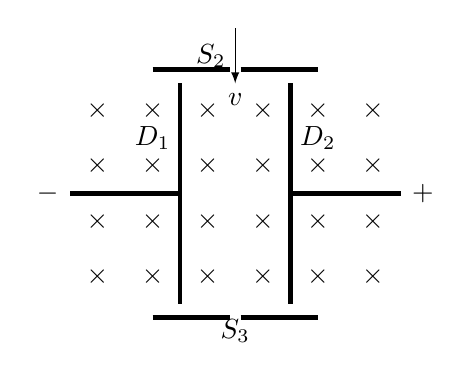
\begin{tikzpicture}[>=latex,scale=0.7]
  \foreach \x in {1,...,6}
	\foreach \y in {1,...,4}
	{
		\node at (\x,\y){$\times$};
	}
\draw [ultra thick] (2.5,0.5)--(2.5,4.5)	;
\draw [ultra thick] (4.5,0.5)--(4.5,4.5)	;
\draw  [ultra thick](2.5,2.5)--(0.5,2.5)node [left]{$-$};
\draw  [ultra thick](4.5,2.5)--(6.5,2.5)node [right]{$+$};
\draw [ultra thick] (2,4.75)--(3.4,4.75);  \draw  [ultra thick](3.6,4.75)--(5,4.75);
\draw  [ultra thick](2,.25)--(3.4,.25);  \draw  [ultra thick](3.6,.25)--(5,.25);
\draw [->](3.5, 5.5)--(3.5, 4.5) node [below]{$v$};
\node at (3.5,5)[left]{$S_2$};\node at (3.5,0){$S_3$};
\node at (2,3.5){$D_1$};\node at (5,3.5){$D_2$};
\end{tikzpicture}
\end{document}